\section{External Processes}
\label{sec:externalprocs}

% External processing jobs can be centrally managed in StreamFS as well.  
In real deployments, %it is often the case that
users do want to be limited by the particular libraries that are available to them in javascript or they have already made
a signficant investment in time writing and testing their own processing jobs.  For them, we provide an external client stub that 
re-directs data from standard in/out through a network connection to/from the StreamFS process manager.  The stub also interprets
process management commands to spawn and kill jobs and associate different subscriptions with different instances of a jobs 
running on the client side.

\begin{figure}[h!] %htbp
\centering
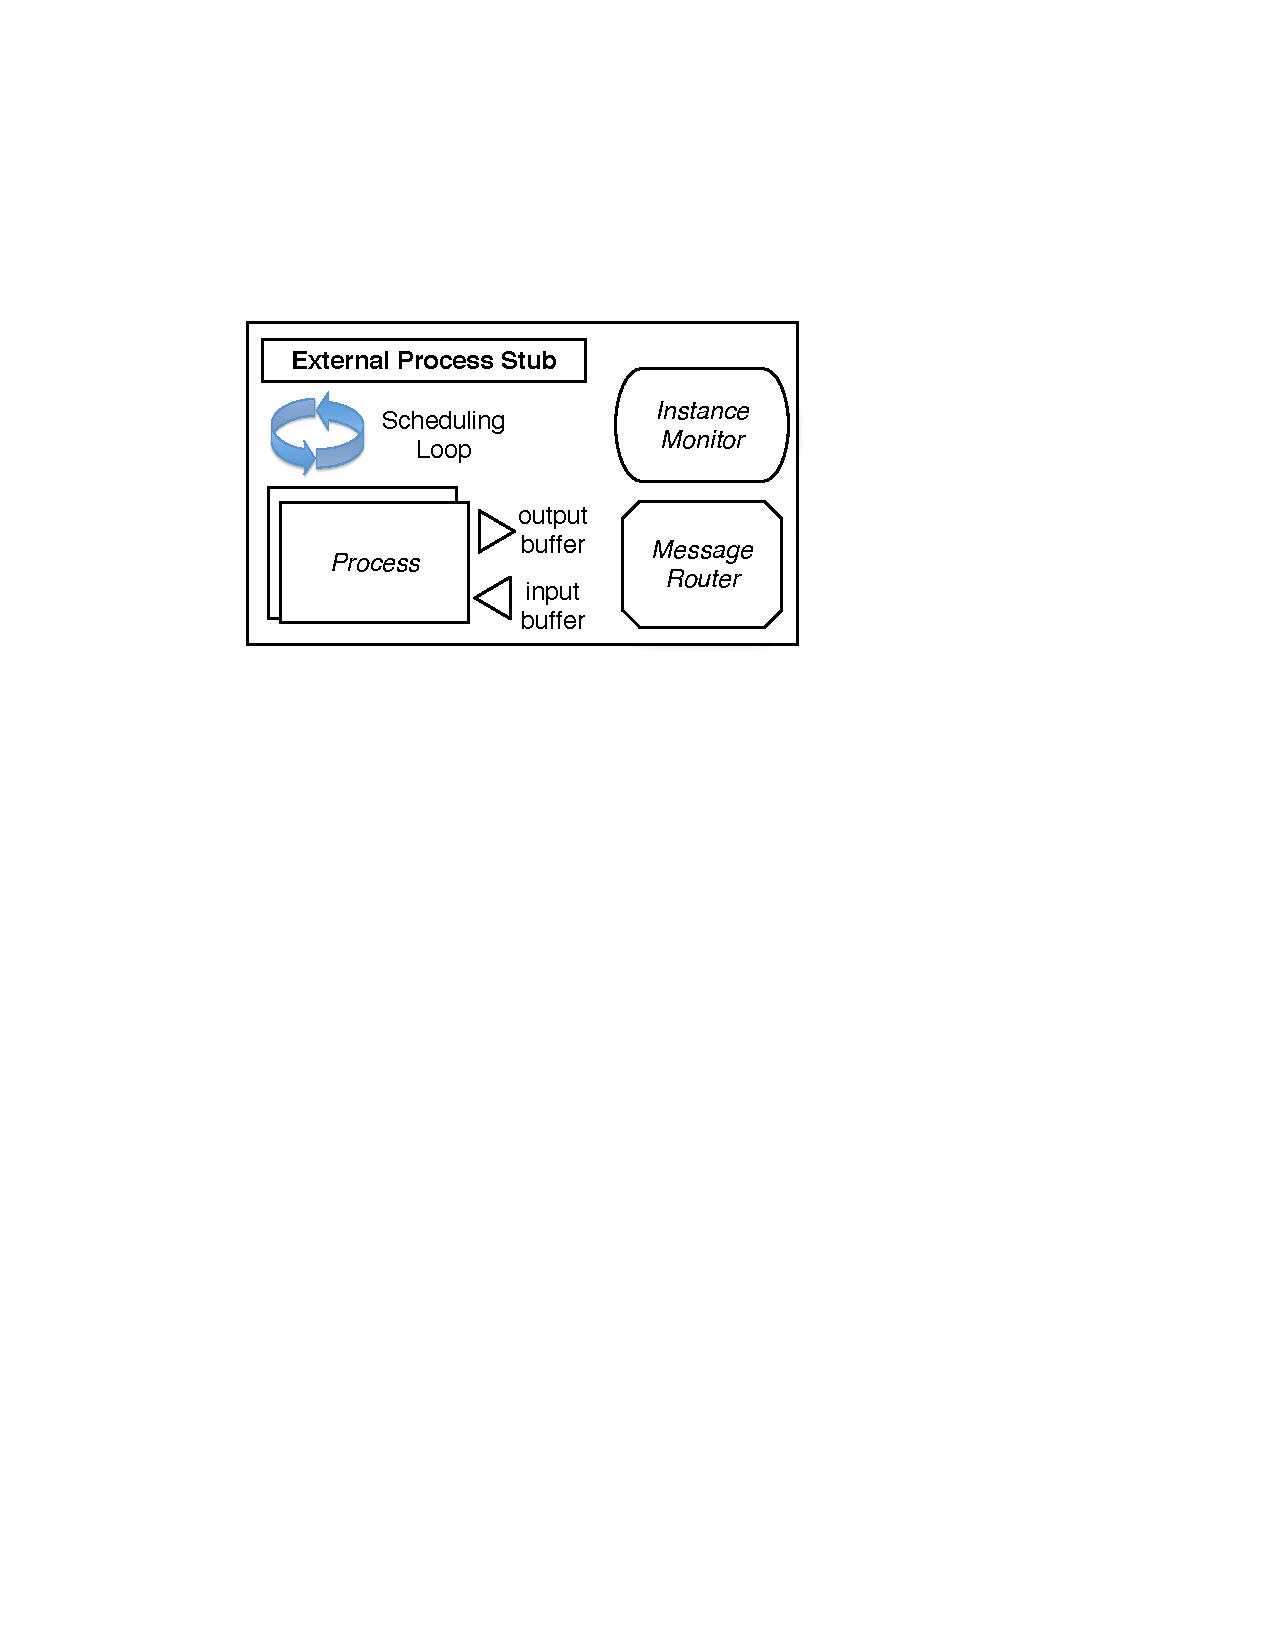
\includegraphics[width=0.55\columnwidth]{figs/external_stub}
\caption{External process stub.  Note, it contains similar component to a process element and functions much the same way, 
managing the buffers, scheduling, errors, and communication on the client side like the PE.}
\label{fig:external_stub}
\end{figure}

Figure~\ref{fig:external_stub} shows the internal components of a client stub.  Note, it contains very similar components to
a process element and work in a similar fashion.  The client stub contains the four major components:

\begin{enumerate}
\item \emph{Scheduler}: The scheduler schedules the execution of jobs on the client machine.  It uses the \texttt{window} and
						\texttt{timeout} parameters to set when and how often the job is set to run.
\item \emph{Process}:  The process component is simply in charge of managing communication with the process that is spawn
						on the local machine.  It maintains an pipe to each local process.  The processes
						run indepdently and share no memory directly.  Data from the input buffer is copied to the 
						pipe connection to the process.
\item \emph{Message Router}: The message router maintains a socket connection to the Process Manager and writes to the associated
								buffer for specific jobs.
\item \emph{Instance Monitor}: The instance monitor re-starts jobs when/if they fail and forward local errors to the process manager
								to annotate the associated files in StreamFS.
\end{enumerate}

On startup, the client stub read a local configuration file that specifies the path to the job and metadata that describes
job.  These are used to register the job with StreamFS and set the metadata attributes.  The registration on the StreamFS 
server is exposed through an \emph{external process} file.  The user interact with an external job exactly the same way they
interact with an internal process job.  In order to spawn a job on the client, the user simply ``pipes'' a stream file 
to the external process file.  The creation of the pipe/subcription send a spawn message to the client and starts the associated
job on the client.  Once the process is started, data from the stream(s) is forwarded to the client, which writes it to the 
standard-in of the client job.  Starting a job also creates a stream file the StreamFS server.  Any data that's produced by the job
and written to standard-out is re-directed to the server and made available through the stream file.

This desgin is consistent with the semantics of pipe/subscription management and functionality.  Recall, internal processes
work the same way and this allow us to stay consistent with the file-centric principal whereby \emph{everything is managed
through the filesystem itself as a file}.


